\documentclass[10pt,conference]{IEEEtran}
% Add the compsocconf option for Computer Society conferences.
\usepackage{mathtools}
\usepackage{amssymb,amsmath}

% Pranav comment this line below to take out all the comments from the paper
\newcommand{\ENABLECOMMENTS}{}

\usepackage[T1]{fontenc}
\usepackage{ifpdf}
\usepackage{url}
\usepackage{tabularx}
\ifpdf
\usepackage[pdftex]{graphicx}
\graphicspath{{figs/}}
\DeclareGraphicsExtensions{.pdf,.png,.jpg}
\else
\usepackage[dvips]{graphicx}

\graphicspath{{eps/}}
\DeclareGraphicsExtensions{.eps}
\fi
\usepackage{float}
%\usepackage[caption=false,font=footnotesize]{subfig}
\usepackage[font=footnotesize]{caption}
\usepackage{subcaption}
\usepackage{setspace}
\usepackage{balance}
\pdfminorversion=6
\hyphenation{op-tical net-works semi-conduc-tor}
\newcommand{\indentitem}{\setlength\itemindent{0pt}}
\usepackage{algorithmic}
\usepackage{algorithm}
\newcommand{\algorithmicinput}{\textbf{Input:}}
\newcommand{\INPUT}{\item[\algorithmicinput]}
\newcommand{\algorithmicoutput}{\textbf{Output:}}
\newcommand{\OUTPUT}{\item[\algorithmicoutput]}
\renewcommand{\algorithmicrequire}{\textbf{Pre Condition:}}
\renewcommand{\algorithmicensure}{\textbf{Post Condition:}}
\floatname{algorithm}{Procedure}
\usepackage{tikz}
\usetikzlibrary{matrix,arrows,circuits.ee,circuits.ee.IEC,shapes.geometric,shapes.misc}
\newcommand{\iap}{\textit{DREMS}}
%\newcommand{\iapfull}{\textbf{D}istributed \textbf{S}oftware \textbf{P}latform }
\newcommand{\iapfull}{\textbf{D}istributed \textbf{RE}altime \textbf{M}anaged \textbf{S}ystem}% Algorithmic modifications
\newcommand{\ALOOP}[1]{\ALC@it\algorithmicloop\ #1%
  \begin{ALC@loop}}
\newcommand{\ENDALOOP}{\end{ALC@loop}\ALC@it\algorithmicendloop}
\renewcommand{\algorithmicrequire}{\textbf{Input:}}
\renewcommand{\algorithmicensure}{\textbf{Output:}}
\newcommand{\algorithmicbreak}{\textbf{break}}
\newcommand{\BREAK}{\STATE \algorithmicbreak}
\usepackage{color}


\ifdefined\ENABLECOMMENTS
\newcommand{\AD}[1]{{\texttt{\color{red}AD:#1}}}
\else
\newcommand{\AD}[1]{}
\fi
\newenvironment{noindlist}
 {\begin{list}{\labelitemi}{\leftmargin=0.1em \itemindent=0em \itemsep=0.3em}}
 {\end{list}}
\usepackage{multirow}

\begin{document}
\title{ Colored Petri Net-based Modeling and Formal Analysis of Component-based Applications }
\vspace{-0.1in}
\author{\IEEEauthorblockN{Pranav Srinivas Kumar, Abhishek Dubey and Gabor Karsai} 
\IEEEauthorblockA{
  ISIS, Dept of EECS, Vanderbilt University, Nashville, TN 37235, USA \\
  Email:\{pkumar, dabhishe, gabor\}@isis.vanderbilt.edu
}
}

% make the title area

\setcounter{page}{1}
\maketitle
\begin{abstract}
%Architecture-oriented domain-specific modeling languages (DSML) can provide a concise and modular abstraction for the structural and behavioral properties of a component-based system. DSMLs are increasingly used in distributed real-time (DRE) systems to manage the complexity and heterogeneity of architectural specifications, both in software and hardware. Such languages also enable model transformations, development automation and design-time analysis before deployment. 

This paper presents a timing analysis approach for modeling and verifying component-based software applications hosted on distributed real-time embedded (DRE) systems. Although schedulability analysis for real-time systems has been a considerably well-studied field, various general-purpose timing analysis tools are not intuitively applicable to all system designs, especially when domain-specific properties such as hierarchical scheduling schemes, time-varying networks and component-based interaction patterns directly influence the temporal behavior. Thus, there is still a need to develop analysis tools that are tightly coupled with the target system paradigm and platform while being generic and extensible enough to be easily modified for a range of systems. In this context, we have developed a Colored Petri Net-based schedulability analysis tool that integrates with a domain-specific modeling language and component model and that simulates and verifies temporal behavior for component operations in mission-critical DRE systems. Our results show the scalable utility of this approach for preemptive and non-preemptive hierarchical scheduling schemes in distributed scenarios.
\end{abstract}

\begin{IEEEkeywords}
	component-based, real-time, distributed, colored petri nets, 
	timing, schedulability, analysis
\end{IEEEkeywords}
\section{Introduction}

Real-time systems, by definition, must meet operational deadlines. These deadlines constrain the amount of time permitted to elapse between a stimulus provided to the system and a response generated by the system. Delayed responses or missed task deadlines can have catastrophic effects on the function of the system, especially in the case of safety- and mission-critical applications. This is the primary motivation for design-time schedulability analysis and verification of systems. 

There is a wealth of existing literature studying real-time task scheduling theory and timing analysis in uniprocessor and multiprocessor systems \cite{Audsley1995, Sha2004}. There are also several modeling, schedulability analysis and simulation tools \cite{MAST1, Cheddar, TIMES, PTIDES} that address various challenges in verifying real-time requirements although many such tools are appropriate only for certain task models, interaction patterns, scheduling schemes, or analysis goals. For component-based architectures, model-based system designs are usually expressed in a formal domain such as timed automata \cite{Alur1994, Macariu2010}, controller automata \cite{Zhang2012}, high-level Petri nets \cite{masri2009} etc. so that existing analysis tools such as UPPAAL \cite{UPPAAL} or CPN Tools \cite{CPNTools} can be used to verify either the entire system or its compositional parts. But, it is also evident that many of the existing schedulability analysis tools, though grounded in theory are not directly applicable to all system designs, especially with respect to domain-specific properties such as component interaction patterns, distributed deployment, time-varying communication networks etc. 

To be useful, the analysis tools need to be tightly integrated with the target domain: the concurrency model used by the system. The classic thread-based concurrency model (with generic synchronization primitives) is too low-level and too generic, it is hard to use, and hard to analyze. For pragmatic reasons, more restrictive, yet useful concurrency models are needed for which dedicated analysis tools can be developed. Our previous efforts \cite{MoDeVVa} were directed at this challenge. The target domain for that study was the DREMS component model \cite{DREMS13Software} which is the foundation of a software infrastructure addressing challenges in the design, development, and deployment of component-based embedded software for distributed applications like flight software for fractionated spacecraft. The physical nature of such systems requires strict, accurate and pessimistic timing analysis at design-time to avoid catastrophic situations at run-time. DREMS is implemented as a design-time tool suite and a run-time software platform that is enhanced by a component (concurrency) model with well-defined execution and interaction semantics. The platform relies on a temporally partitioned task scheduling scheme, a non-preemptive component-level operations scheduler, support for various communication and interaction patterns; all deployed on a distributed hardware platform.

Our contributions in this paper target efficient modeling and analysis techniques of temporal behavior for component-based applications that form distributed real-time embedded systems, such as DREMS. 

\begin{enumerate}
	\item We present an approach for modeling  the 'business logic': the operational behavior of each component in an application. The model uses a sequence of timed steps that are executed in the course of a component operation, including steps that specify interactions with other components. This approach enables abstracting the details of the middleware, while representing the temporal behavior of the component business logic. 
	\item We also present improvements to the CPN-based modeling approach that enables better analysis performance and scalability. These rely on heuristics that manage time variables and state space data structures more efficiently. 
	\item We also present advanced state space analysis methods and tools applied on the modeled system to reduce analysis time on medium to large-scale systems.
\end{enumerate}

The rest of this paper is organized as follows. Section \ref{sec:Related_Research} presents related research, reviewing and comparing existing analysis tools and formal methods. Sections \ref{sec:Target_System_Architecture} briefly describes the DREMS architecture, specifically the concepts of interest that are covered by the timing analysis tool. Section \ref{sec:Modeling} describes the business logic modeling approach to capture the operational behavior of components in the application. Section \ref{sec:Analysis} describes the analysis improvements we were able to achieve with structural changes to the analysis model. This section also briefly describes the application of advanced state space analysis methods that enable efficient state space searches while reducing the state space size and overall memory consumption. Section \ref{sec:Future_Work} evaluates possible extensions to this work before concluding with Section \ref{sec:Conclusions}.
\vspace{-0.05in}

\section{Related Research}
\label{sec:Related_Research}

In recent years, much of the proliferating work in the development of mission-critical distributed real-time systems addresses the need for Safety and Verification-driven Engineering. Structural properties of the system are established using domain-specific modeling tools. Design models are transformed into relevant analysis models to study probable behaviors of the system and identify anomalies. When analyzing timing behavior, typically several exaggerated assumptions are made about the system behavior. These include upper bounds on task execution times, service rates, maximum resource consumption etc. The results of system analysis using such assumptions are equally pessimistic. However, real-time systems with high criticality necessitate such pessimistic assumptions to avoid the consequences of poor design. Predictability of system behavior is achieved by obtaining upper bounds of the system properties.   

Petri nets and their extensions have proven to be a powerful formalism for modeling and analyzing concurrent systems. System designs represented using a domain-specific modeling languages are often translated into Petri nets for formal analysis. High-level formalisms such as AADL models have been translated into Symmetric nets for qualitative analysis \cite{kordon_sn} and Timed Petri nets \cite{kordon2009} to check for real-time properties such as deadline misses, buffer overflows etc. Similar to \cite{kordon2009}, our CPN-based analysis also makes use of observer places \cite{Alpern1989} that monitor the system behavior and look for real-time property violations and prompt completion of operations. However, \cite{kordon2009} only considers periodic threads in systems that are not preemptive. Our analysis covers a broader range of thread interaction patterns geared towards component-based applications operating on a hierarchical scheduling scheme requiring higher-level modeling concepts to capture component interaction in a distributed setup. 

%\AD{since you are discussing hierarchical scheduling here - you should describe the system or the framework briefly in the introduction.}

In the context of component-based systems, for complete real-time analysis, it is necessary to obtain significant information about the component assembly, the interaction patterns and real-time data about the temporal behavior of components. The real-time model of the system is composed of real-time models of its constituent parts, each with its own temporal behavior. Using abstract model descriptors, \cite{Lopez2006} describes a real-time model for component-based systems, including semantic and quantitative meta-data about component real-time behavior. Using the MAST transactional modeling methodology \cite{MAST1, MAST2} and analysis tools in the MAST environment, schedulability checks and priority assignment automation are performed. It must be noted here that for every real-time application, a separate and independent real-time analysis model is generated for each mode of operation and analyzed separately.

%Several analysis approaches present tool-aided methodologies that exploit the capabilities of existing analysis and verification techniques. In the verification of timing properties of composed systems, \cite{medina2011} uses the OMG UML Profile for Modeling and Analysis of Real-Time and Embedded Systems (MARTE) modeling standard with model transformations to convert design models into MAST output models for concrete schedulability analysis. In a similar effort, AADL models are translated into real-time process algebra \cite{sokolsky2006} reducing schedulability analysis into a deadlock detection problem searching through state spaces and providing failure scenarios as counterexamples.

%In order to analyze hierarchical component-based systems, the real-time resource requirements of higher-level components need to be abstracted into a form that enables scalable schedulability analysis. The authors in \cite{easwaran2006} present an algorithm where component interfaces abstract the minimum resource requirements of the underlying components, in the form of periodic resource models. Using a single composed interface for the entire system, the component at the higher level selects a value for operational period that minimizes the resource demands of the system. Such refinement is geared towards minimum waste of system resources. 

For classes of component-based systems whose component assembly and application structure change dynamically over time, design-time verification is observed to be insufficient. Incremental re-verification strategies \cite{johnson2013} have been applied on dynamic systems to augment traditional compositional verification by identifying the minimal set of components that require re-verification after dynamic changes. Since our approach considers design-time deployment plans that are static, the analysis does not consider dynamic changes to component assembly at run-time. 

\vspace{-0.1in}
\section{Background}
\label{sec:Background}

\subsection{DREMS Infrastructure}
%\subsubsection{The Component Model}
%\label{sec:The_Component_Model}

%The DREMS platform is characterized by a hierarchical scheduling scheme. The higher, component-level scheduler schedules component operations for execution, enabling interactions between application components. The lower, operating system scheduler enforces a temporal partitioning scheme and schedules the component threads. Components are grouped into unique, identifiable processes called actors. These actors are assigned to temporal partitions and run only when the associated temporal partition is active. This partitioned scheduling provides a guaranteed slice of the CPU to all the actors and enables isolation between multiple applications running on the same computing node.

\subsubsection{DREMS Components}
\label{sec:drems_component}
%\vspace{0.1in}
Design and implementation of component-based software applications rests on the principle of assembly: \textit{Complex systems can be built by composing re-useable interacting components}. Components contain functional, business logic code that implements operations on state variables. Ports facilitate interactions between communicating components. A component-level message queue, with associated infrastructure code, controls the scheduling of operations on the individual components. Figure \ref{fig:drems_component} shows a basic DREMS component.  

%\vspace{-0.07in}
\begin{figure}[ht]
\centering
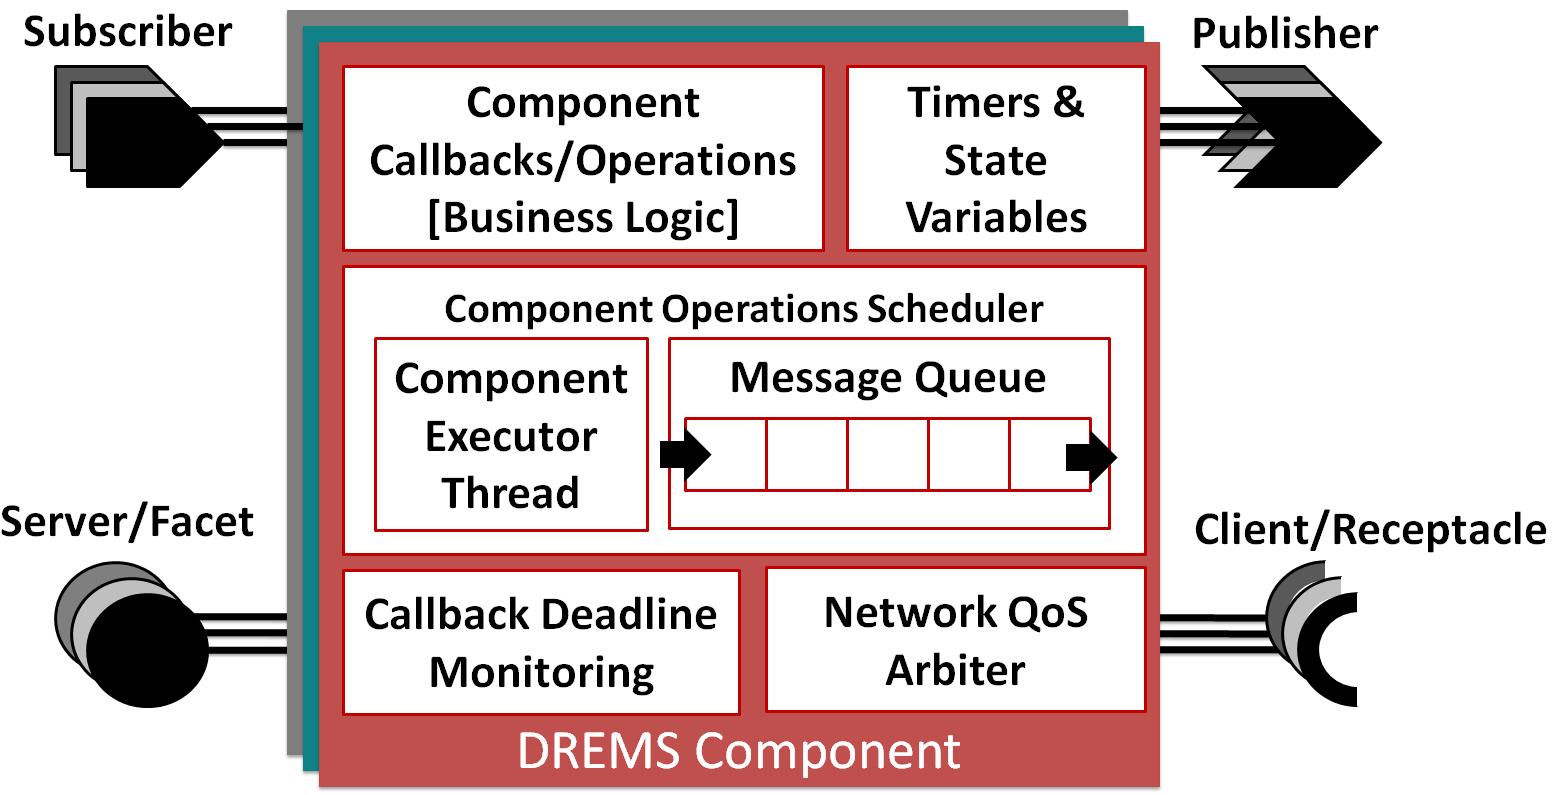
\includegraphics[width=0.35\textwidth]{drems_component}
\caption{DREMS Component}
\label{fig:drems_component}
\vspace{-0.2in}
\end{figure}
\vspace{0.1in}

Each DREMS component supports four basic types of ports for interaction with other collaborating components: Facets, Receptacles, Publishers and Subscribers. A component's {\bf facet} is a unique interface that it exposes to its clients. This interface can be invoked either synchronously via remote method invocation (RMI) or asynchronously via asynchronous method invocation (AMI). A component's {\bf receptacle} specifies an interface required by the component in order to function correctly. Using its receptacle, a component can establish connections and invoke operations on other components using either RMI or AMI. A {\bf publisher} port is a single point of data emission. This port emits data produced by a component operation. A {\bf subscriber} port is a single point of data consumption, feeding received data to the associated component. Communication between publishers and subscribers is contingent on the compatibility of their associated topics. Publishers and Subscribers enable the OMG DDS anonymous publish/subscribe style of messaging. More details on this component model can be found in ~\cite{ISIS_F6_ISORC:13}.

%Additionally, this component model also supports sporadic and periodic timers that can be used to initiate component operations. 


\subsubsection{Component Operations}
\label{sec:component_operations}
An operation is an abstraction for the different tasks undertaken by a component. These tasks are implemented by the component's executor code written by the developer. In order to service interactions with the underlying framework and with other components, every component is associated with a message queue. This queue holds instances of operations ('messages') that are ready for execution and need to be serviced by the component. These operations service either interaction requests (seen on communication ports) or service requests (from the underlying framework). An example for the latter is the use of component timers that can periodically (or sporadically) activate an operation. 

Figure \ref{fig:component_operations} shows the basic structure of this model. Each operation is characterized by a priority and a deadline. Operation deadlines are quantified in absolute time measured starting from when the operation is enqueued onto the component message queue. %These operations are sorted and scheduled based on one of three scheduling schemes: Earliest Deadline First (EDF), First In First Out (FIFO), and Priority FIFO. 

\vspace{-0.12in}
\begin{figure}[ht]
\centering
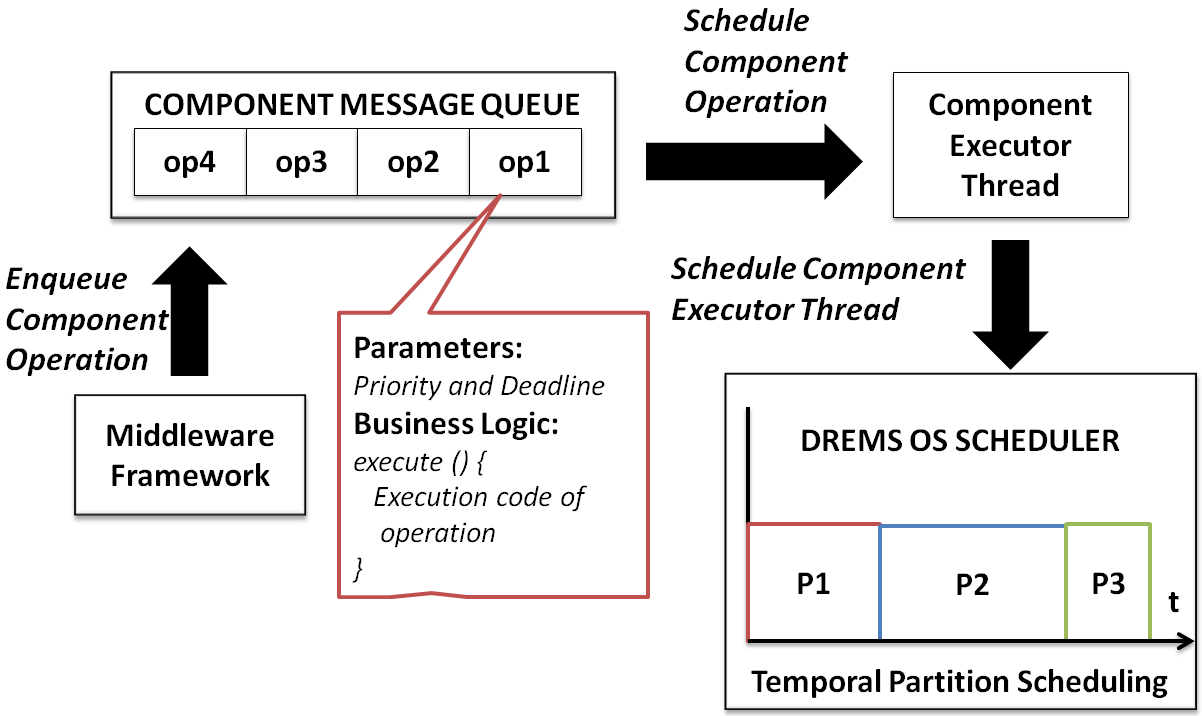
\includegraphics[width=0.4\textwidth]{component_operations}
\caption{Scheduling Component Operations}
\label{fig:component_operations}
\vspace{-0.18in}
\end{figure}
%\vspace{0.2in}

To facilitate component behavior that is free of deadlocks and race conditions, the component's execution is handled on a single thread. Operations in the message queue are therefore scheduled one at a time under a non-preemptive policy. A component dispatcher thread dequeues the next ready operation from the component message queue. This operation is scheduled for execution on a component executor thread. The operation is run to completion before another operation from the queue is serviced. This single-threaded execution helps avoid synchronization primitives such as internal state variables that lead to strenuous code development. Though components that share a processor still run concurrently, each component operation is executed on a single component-specific executor thread.

Figure \ref{fig:timing_diagram} shows a sample timing diagram of how a component operation is handled. At time 0, the component executor thread is running some previously ready component operation, \emph{op1}. At this point, consider that a new component operation \emph{op2} is enqueued onto the message queue and marked as ready. At time 10, assuming that no other component requires scheduling, the component dispatcher thread of this component dequeues the next ready operation for execution. Assuming the component executor thread is scheduled immediately by the underlying processor, this thread runs the ready operation by invoking its \emph{execute} function. This operation is run to completion at time 16. The total time taken for execution of this operation is measured from when the operation was enqueued, i.e. time 0. If the time taken for the operation exceeds its deadline, a fault manager is immediately notified. The duration of the component operation is further delayed by temporal partitioning enforced by the OS scheduler. This adds to the need for schedulability analysis, especially in case of safety and mission-critical applications.

\begin{figure}[ht]
\centering
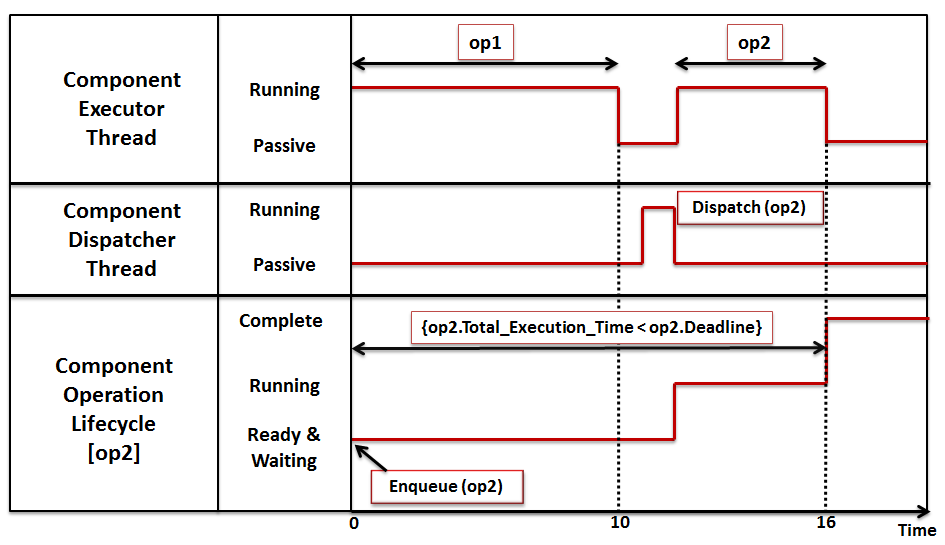
\includegraphics[width=0.50\textwidth]{cop_timing_diagram}
\caption{Component Operation Execution}
\label{fig:timing_diagram}
\vspace{-0.2in}
\end{figure}
\vspace{0.1in}

\subsubsection{Temporal Partition Scheduler}
\label{sec:Temporal_Partition_Scheduler}

DREMS components are grouped into processes that are assigned to temporal partitions, implemented by the DREMS OS scheduler. This scheduler was implemented by modifying the behavior of the standard Linux scheduler, introducing an ARINC-653 ~\cite{ARINC-653} style temporal and spatial partitioning scheme. 

\vspace{-0.12in}
\begin{figure}[ht]
\centering
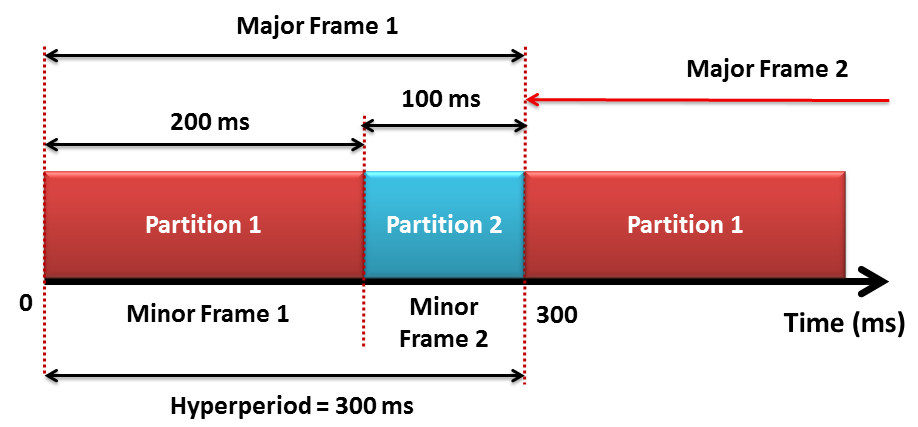
\includegraphics[width=0.37\textwidth]{partition_scheduling}
\caption{Sample Temporal Partition Schedule with Hyperperiod = 300 ms}
\label{fig:partition_scheduling}
\vspace{-0.1in}
\end{figure}


% THis is probablky not needed - the only relevant topic here is temporal partitioning.
%The scheduler further groups threads into different criticality levels: Critical, Application, and Best-Effort. Critical threads handle system and mission management tasks; Application-level threads include component executor threads that perform mission-specific non-critical tasks; Best-Effort threads handle low priority tasks that are scheduled only when there are no other runnable threads from the other two categories.
Temporal partitions are periodic fixed intervals of the CPU's time. Threads associated with a partition are scheduled only when the partition is active. This enforces a temporal isolation between threads assigned to different partitions. The repeating partition windows are called \emph{minor frames}. The aggregate of repeating minor frames is called a \emph{major frame}. The duration of a major frame is called the \emph{hyperperiod}, which is typically the lowest common multiple of the partition periods. Each minor frame is characterized by a period and a duration. The period indicates how often this partition becomes active and the duration indicates how much of the CPU time is available for scheduling the runnable threads associated with that partition. Temporal partitions with fixed periods and durations are chosen such that a valid execution schedule is realized by their coexistence. Figure \ref{fig:partition_scheduling} shows a sample temporal partition schedule. 

%This schedule is made up of two minor frames. Assuming the schedule is enforced at time t = 0, partition 1, characterized by minor frame 1, is made active by the partition scheduler. This partition stays active for the duration of the minor frame, 200 ms. At this point, partition 1 is deactivated and partition 2, characterized by minor frame 2, is activated. Partition 2 stays active for 100 ms, after which the major frame ends and the schedule is repeated.

\subsection{Colored Petri Nets}

Petri nets \cite{Murata1989} are a graphical modeling tool used for describing and analyzing a wide range of systems. A Petri net is a five-tuple $(P, T, A, W, M0)$ where P is a finite set of places, T is a finite set of transitions, A is a finite set of arcs between places and transitions, W is a function assigning weights to arcs, and M0 is the initial marking of the net. Places hold a discrete number of markings called tokens. Tokens often represent resources in the modeled system. A transition can legally fire when all of its input places have necessary number of tokens. 
% Simplify...
%Since Petri net tokens are not distinguishable, the obtained model is often too complex for large systems. To enable compact representations for the modeled system, extensions to the basic Petri net model, called high-level Petri nets, are preferred.
With Colored Petri nets (CPN) \cite{CPN}, tokens contain values of specific data types called colors. Transitions in CPN are enabled for firing only when valid colored tokens are present in all of the typed input places, and valid arc bindings are realized to produce the necessary colored tokens on output places. The firing of transitions in CPN can check for and modify the data values of these colored tokens. Furthermore, large and complex models can be constructed by composing smaller sub-models as CPN allows for hierarchical description. This extended paradigm can more easily model and analyze systems with typed parameters. 


\section{Problem Statement}
\label{sec:Problem_Statement}

\vspace{-0.05in}
Consider a set of mixed-criticality component-based applications that are distributed and deployed across a cluster of embedded computing nodes. Each component has a set of interfaces that it exposes to other components and to the underlying framework. Once deployed, each component functions by executing operations observed on its component message queue. Each component is associated with a single executor thread that handles these operation requests. These executor threads are scheduled in conjunction with a known set of highly critical system threads and low priority best-effort threads. Furthermore, the application threads are also subject to a temporally partitioned scheduling scheme. System assumptions include (1) knowledge on the sequence of computational steps of known duration that are executed inside each component operation, (2) knowledge on the worst-case estimated time taken on each computational step, and (3) the worst-case estimated times taken to invoke a remote function and to process a response, accounting for network-level delays. Using this knowledge about the system, the problem here is to ensure that the temporal behavior of all the application components lie within the bounds laid out by the system specifications. Ideally, this is achieved by verifying system properties like lack of deadline violations for component operations. For scenarios where the system design isn't complete, e.g. application thread priorities are unknown, the paper investigates the utility of the approach in identifying the subset of system behaviors that satisfy timing requirements and provide useful information to designers, e.g. partial thread execution orders. %Equally important is the problem of identifying a formal domain that is easily extensible and scalable for larger systems.   

\section{Colored Petri Net-based Analysis Model}
\label{sec:CPN_Modeling}

This section briefly describes how CPN can be used to build an extensible, scalable analysis model for component-based software applications. %In the context of the component model and the OS scheduler described in Section \ref{sec:Background}, this involves capturing (1) the nature of temporal partitioning, (2) properties of the component executor threads, (3) priority-based scheduling of the component executor threads, and finally, (4) using knowledge of the component's business logic code to model the scheduling of component operations. 
To edit, simulate and analyze this model, we use the CPN Tools 4 \cite{CPNTools} tool suite.  

\subsection{Model of Time}
\label{sec:model_of_time}

Appropriate choice for temporal resolution is a necessary first step in order to model and analyze threads running on a processor. The lowest-level OS scheduler enforces temporal partitioning and uses a priority-based scheme for threads active within a partition. The highest priority ready thread is always chosen first for execution. This thread keeps hold of the CPU as long as it is runnable and there are no other threads of same priority that need to run. If multiple threads have the same priority, Round-Robin (RR) scheduling  is enforced. Here, the scheduler allots a small quantum of time to one of the ready threads after which the thread is preempted by another ready thread of same priority. In order to observe and analyze this behavior, we have chosen the temporal resolution to be 1 ms (a fraction of 1 clock tick of the system timer). Since the temporal resolution is set as a global integer variable in the model, this value can be raised or lowered depending on the nature of the system being analyzed. 

\subsection{Modeling Temporal Partition Scheduling}
\label{sec:Modeling_Temporal_Partition_Scheduling}

Figure \ref{fig:cpn_tps} shows how the temporal partitioning is modeled using CPN. Each minor frame is modeled as a record color-set consisting of a partition number, a period, a duration and an offset. Aggregate of such minor frame tokens can fully describe a partition schedule. Complete partition schedules are maintained per computing node.

\vspace{-0.08in}
\begin{figure}[ht]
\centering
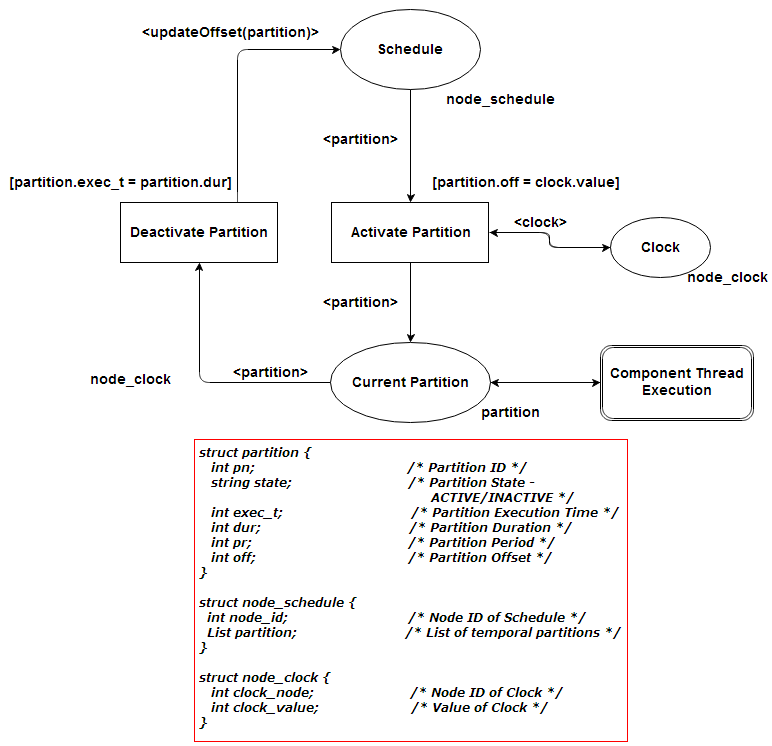
\includegraphics[width=0.40\textwidth]{cpn_tps}
\caption{CPN Model for Temporal Partition Scheduling}
\label{fig:cpn_tps}
\vspace{-0.2in}
\end{figure}
\vspace{0.05in}

Assuming that the partition scheduling shown in Figure \ref{fig:partition_scheduling} is imposed on the OS scheduler in node 1, the \emph{node\_schedule} token corresponding to this schedule is shown in Figure \ref{fig:cpn_tps_token}. This token populates the \emph{Schedule} place and decides the order of partition scheduling. When the node clock reaches the offset of one of these partitions, a valid binding is realized in order to fire the \emph{Activate Partition} which chooses the appropriate partition token and declares it as the \emph{Current Partition}. This active partition behaves as a constraint on the set of runnable component executor threads. \emph{Component Thread Execution} is a hierarchical transition that handles execution of component threads 1 ms at a time. At each millisecond, the \emph{exec\_t} field of the partition is updated. When this count reaches the duration of the partition, the offset of the partition is incremented by its period and the partition is made inactive. The above sequence of steps repeats for each partition.

\vspace{-0.08in}
\begin{figure}[ht]
\centering
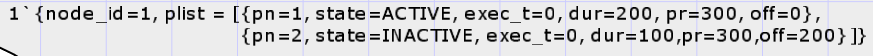
\includegraphics[width=0.5\textwidth]{cpn_tps_token}
\caption{CPN Token corresponding to Figure \ref{fig:partition_scheduling}}
\label{fig:cpn_tps_token}
\vspace{-0.18in}
\end{figure}
%\vspace{0.1in}
   
\subsection{Modeling Component Thread Behavior}
\label{sec:Modeling_Component_Thread_Lifecycle}

Figure \ref{fig:cpn_ctecycle} presents a simplified version of the CPN to model the thread execution cycle. The place \emph{Component\_Threads} holds \emph{node\_threads} tokens that keep track of all the ready threads in each computing node. Each thread is a record characterized by the node ID, thread ID, partition number, priority, start time of execution and state of currently executing operation. If multiple threads belonging to the same temporal partition are ready, the highest priority thread is chosen for execution. 

If the the highest priority thread is not already servicing an operation request, the highest priority operation from the \emph{Component Message Queue} is dequeued and scheduled for execution. The scheduled thread is placed in \emph{Currently Running Thread}. The guard on \emph{Schedule Thread} ensures that the highest priority ready thread belonging to the \emph{Current Partition} is always scheduled first. 

When a thread token is placed in \emph{Currently Running Thread}, the model checks to see if the thread execution has any effect on itself or on other threads. For instance: When the thread executes an operation that performs an RMI call, the effect of completion of the query is that the thread is moved to a blocked state and cannot run again till it receives a response from the server running on another thread. Such state changes are updated by the model using the \emph{Execute Thread} transition which also progresses time by 1 ms each time it fires. Keeping track of the node clock value, the thread is preempted at each clock tick. This loop repeats as long as there are no complete deadlocks in the system. 

\begin{figure*}
\centering
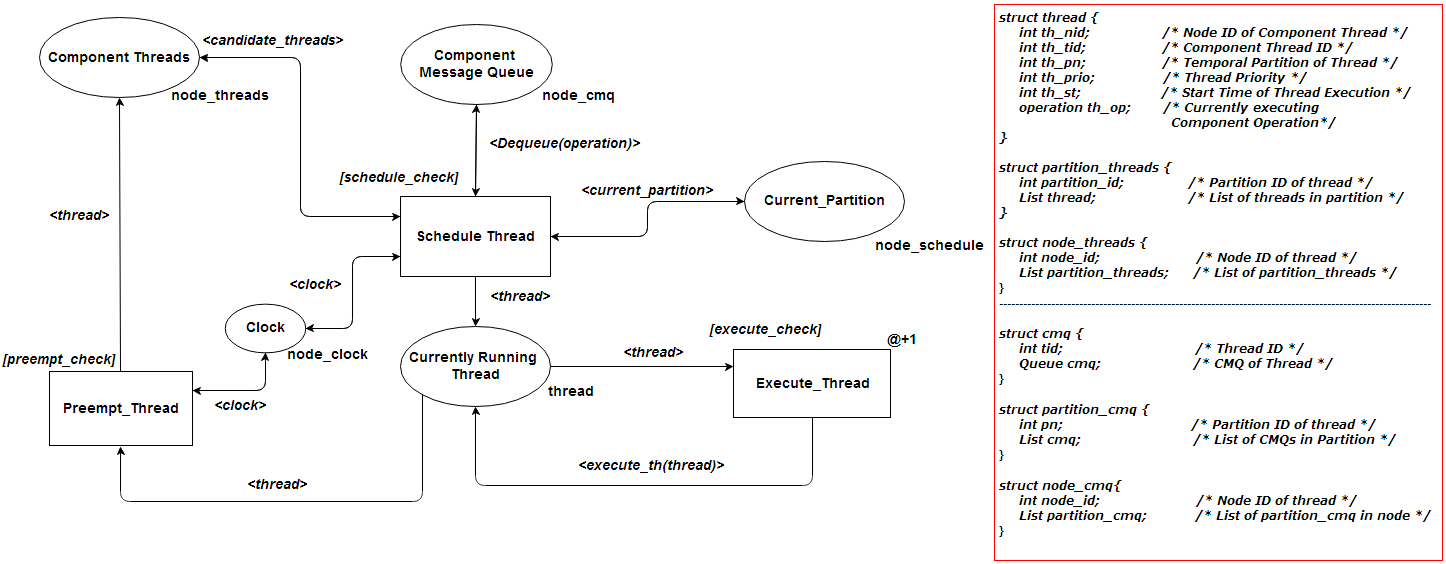
\includegraphics[width=\textwidth]{cpn_ctecycle}
\caption{Component Thread Execution Cycle}
\label{fig:cpn_ctecycle}
\vspace{-0.2in}
\end{figure*}

\subsubsection{Timer Operations}
\label{sec:Timer_Operations}

DREMS components are dormant by default. Once deployed, a component executor thread is not eligible to run until there is an operation added to the component's message queue. 

To start a sequence of component interactions, periodic or sporadic timers can be setup to trigger a component. When the component's timer expires, a timer-related operation is placed on the component message queue. When the component executor thread is picked by the OS scheduler, this operation is dequeued and the timer callback is executed. In CPN, timer operations are modeled as shown in Figure \ref{fig:cpn_timers}. 

\begin{figure}[ht]
\centering
\vspace{-0.1in}
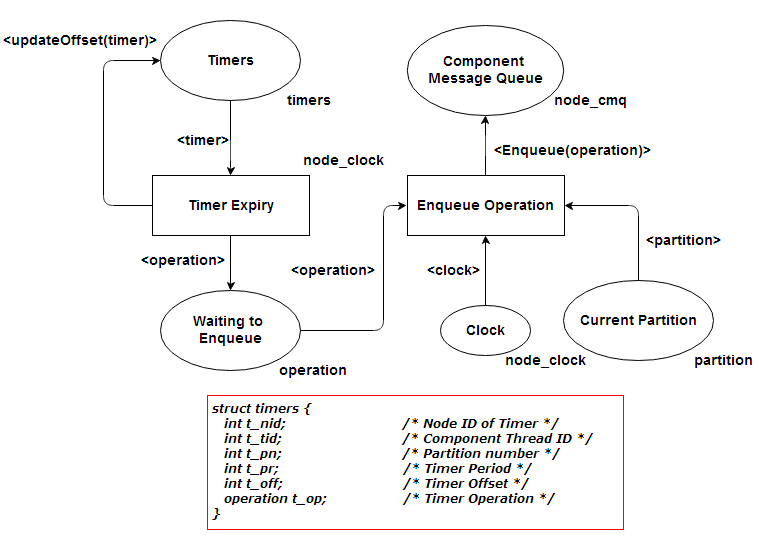
\includegraphics[width=0.5\textwidth]{cpn_timers}
\caption{Timer Operations}
\label{fig:cpn_timers}
\vspace{-0.17in}
\end{figure}

Every timer color-set token consists of a node ID, a thread ID, partition number, a period, an offset relative to the global node-specific clock, and an associated operation. The node ID, thread ID and partition number are necessary to correctly handle the enqueue action. All the component timers are expressed as separate tokens and initialized in the \emph{Timers} place. Notice that the enqueue operation does not happen until the appropriate partition is active. This is because the component-specific thread responsible for enqueueing incoming operations is also affected by temporal partitioning. 

\subsection{Modeling Component Operations}
\label{sec:Modeling_Component_Operations}

\vspace{-0.1in}
\begin{figure}[ht]
\centering
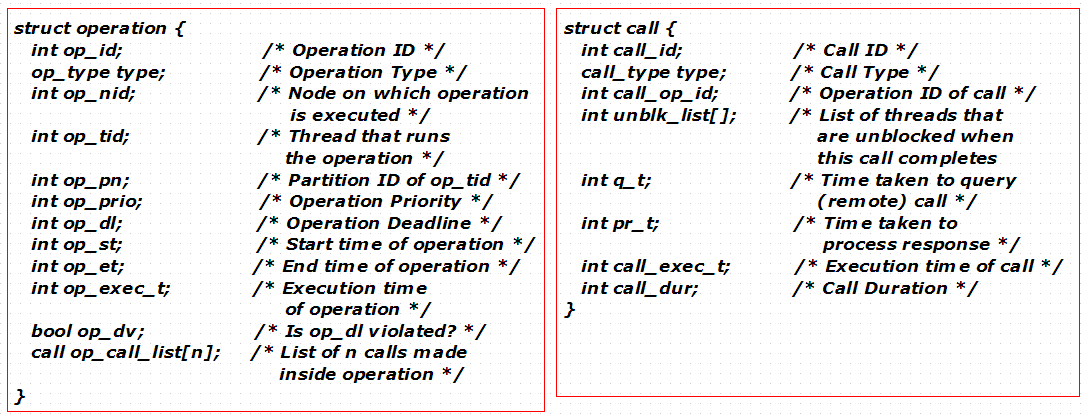
\includegraphics[width=0.5\textwidth]{cpn_operations}
\caption{Color-set for Component Operations}
\label{fig:cpn_operations}
\vspace{-0.2in}
\end{figure}
\vspace{0.1in}

As shown in Figure \ref{fig:cpn_operations}, every component operation is modeled as a record color-set in CPN. This record consists of the operation ID, operation type, node ID, thread ID, partition number, priority, deadline, temporal behavior and a list of function calls that represent the business logic of the execute function. New operations are inserted into the component message queue based on priority. The time stamp \emph{op\_st} is a snapshot of the node clock value when the operation is enqueued onto the message queue. The time stamp \emph{op\_et} is a snapshot of the node clock value when the operation is completed. Accounting for the wait-time in the message queue, the total execution time of the operation is compared against its deadline \emph{op\_dl}.

Once an operation is dequeued, the execution of the operation can be treated as a transition system that runs through a sequence of function calls dictating its behavior. Any of these underlying function calls can have a state-changing effect on the thread executing this operation. Consider a simple RMI application show in Figure \ref{fig:rmi_application}. The application has two components, a client and a server. The client component is associated with a timer that triggers a sequence of interactions between the two components. When the client timer expires, a timer operation is enqueued on the client's operation queue. When scheduled, the client executor thread executes this operation, which makes an RMI call to the server component. Once the query is made, the client thread is effectively blocked till a response is received. The server thread that produces this response may not be scheduled immediately due to the constraints of temporal partition scheduling. Once the RMI operation is completed on the server, the client thread is unblocked. 

\begin{figure}[ht]
\centering
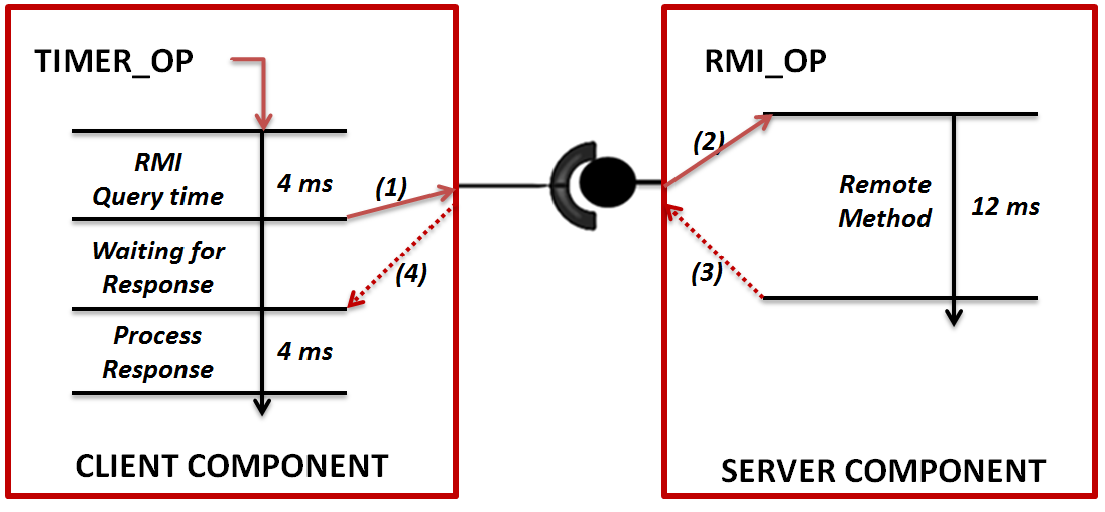
\includegraphics[width=0.4\textwidth]{rmi_application}
\caption{RMI Application}
\label{fig:rmi_application}
\vspace{-0.2in}
\end{figure}
\vspace{0.1in}

In the above example, the duration of time for which the client is blocked, is dependent on what happens inside the remote method on the server. This remote method could either simply take up CPU time, interact with the underlying framework or interact with other components in the application. To capture such interaction patterns, the \emph{call} color-set (Figure \ref{fig:cpn_operations}) is defined in CPN. Each call is identified by a \emph{call\_id} and a \emph{call\_type}. The field \emph{unblk\_list} is a list of threads that are unblocked when the call completes. This field is applicable to the RMI call completion on the server side which unblocks the client thread. Temporal behavior is captured using the last four fields: \emph{q\_t} is the worst-case estimate time taken for completion of a query; \emph{pr\_t} is the worst-case estimate time taken to process a response; \emph{call\_dur} is the effective duration of the call and \emph{call\_exec\_t} keeps track of how much of the call is complete. 

In the context of the earlier RMI example, two \emph{operation} tokens are required to describe the operations handled by the components: a client side timer operation and a server side RMI operation. A sample client timer operation is shown in Figure \ref{fig:cpn_rmi_app_timer_token}.

\vspace{-0.08in}
\begin{figure}[ht]
\centering
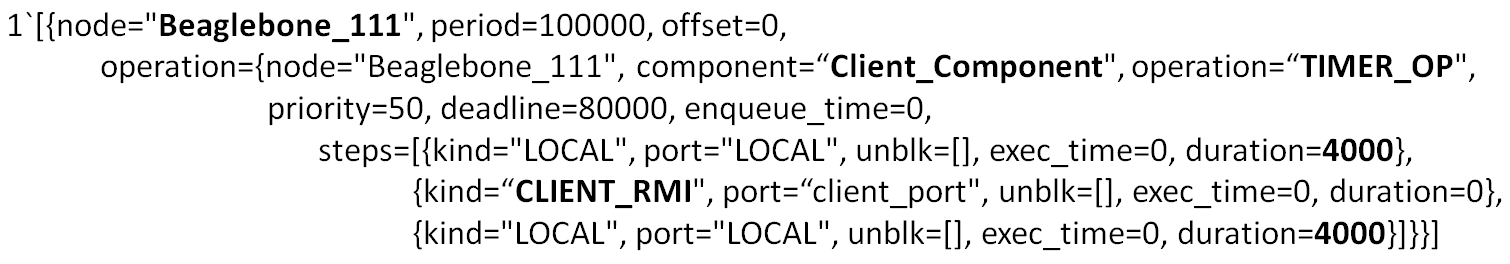
\includegraphics[width=0.5\textwidth]{cpn_rmi_app_timer_token}
\caption{RMI Application - Client Timer Operation}
\label{fig:cpn_rmi_app_timer_token}
\vspace{-0.16in}
\end{figure}


This timer operation runs on the client component (thread 1, partition 1) with a priority of 50, and a deadline of 80 ms. The business logic of this operation consists of a single RMI call that takes 4 ms to send out the query after which it blocks the executing client thread. After the client thread runs for time \emph{t = q\_t}, the client thread is moved to a blocked state and an RMI operation is induced on the server side. The client side thread remains blocked until the server thread completes executing the remote method. Once the server thread completes execution, it sends the response of the RMI back to the client. The model takes note of how long the client has been blocked by using the time stamp at which it receives a response. The client thread runs for an additional \emph{t = pr\_t} to process this response before it marks completion. The token for the server RMI operation is shown in Figure \ref{fig:cpn_rmi_app_server_token}.

%\vspace{0.1in}

This RMI operation is run on the server component (thread 2, partition 2) with a priority of 50 and a deadline of 80 ms. The deadline of this operation cannot be worse than the deadline of the client side operation that initiated the interaction. If this operation delays past 80 ms, a client side deadline violation is realized as the client thread is blocking for longer than expected. 

\vspace{-0.08in}
\begin{figure}[ht]
\centering
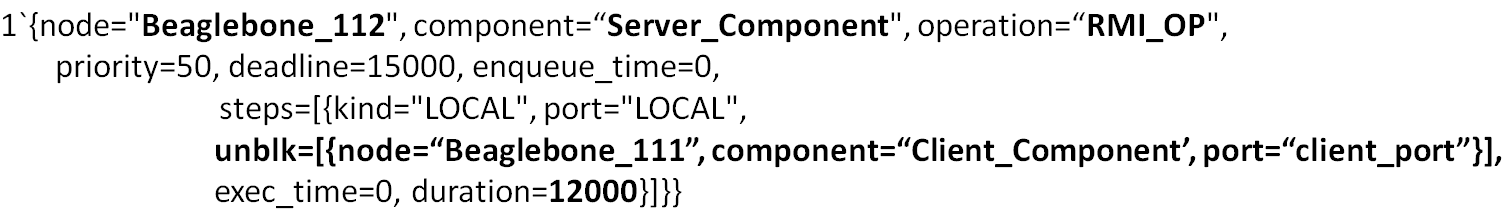
\includegraphics[width=0.5\textwidth]{cpn_rmi_app_server_token}
\caption{RMI Application - Server Operation}
\label{fig:cpn_rmi_app_server_token}
\vspace{-0.14in}
\end{figure}

\subsubsection{Induced Operations}
\label{sec:Operation_Induction}

To handle interactions between components, we take advantage of the developer's knowledge of the structure of the application, i.e, the component wiring. In the earlier example, we know that when the client executes an instance of a timer operation, a related RMI operation is enqueued on the server. In reality, this is handled by the underlying middleware. Since we do not model the details of this framework as of now, Figure \ref{fig:cpn_iop} shows how the CPN model induces operations on components based on the state of the currently running thread. 

Every \emph{induced\_operation} token contains a call ID and an operation. The transition \emph{Induce} observes the activity on the currently running thread. When initiating the model, if a particular call executed by a component thread would, on completion, request the services of another component, a token is placed on the \emph{Induce Operation} place. 

\vspace{-0.06in}
\begin{figure}[ht]
\centering
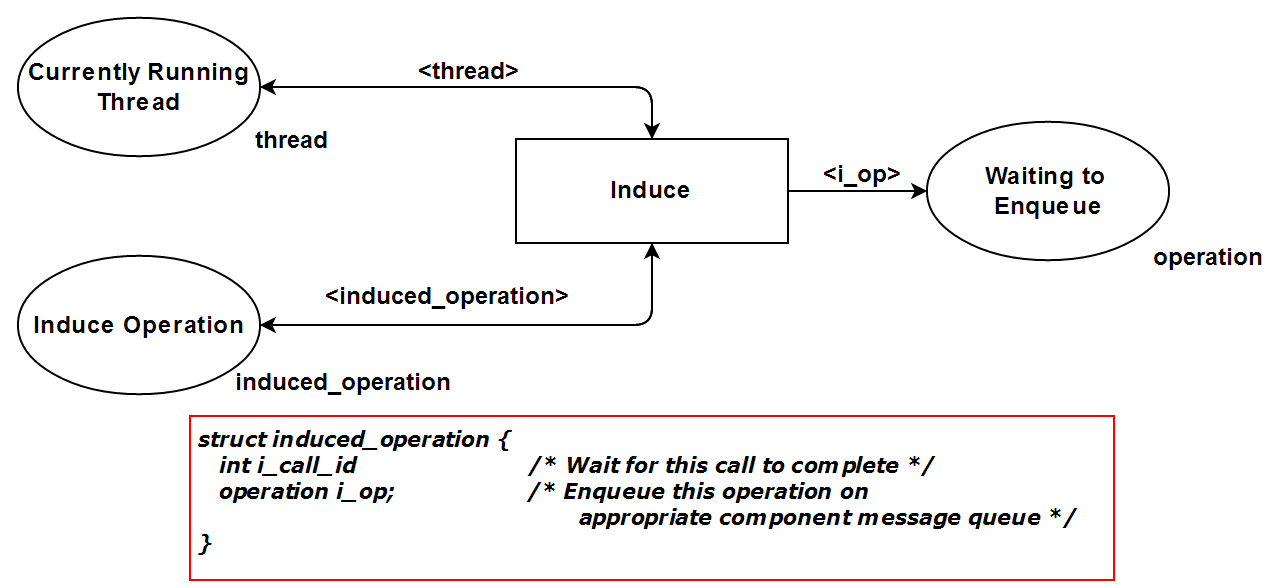
\includegraphics[width=0.5\textwidth]{cpn_iop}
\caption{Operation Induction}
\label{fig:cpn_iop}
\vspace{-0.14in}
\end{figure}
%\vspace{0.1in}

For the earlier RMI example, once the client thread pushes out an RMI query, an operation needs to be induced on the server queue. So an \emph{induced\_operation} token for this interaction is constructed. The model waits for the RMI call on the client side (call ID 1) to complete, at which point it places the operation \emph{i\_op} on the server message queue. This induction is represented in Figure \ref{fig:cpn_rmi_app_iop}. 

\vspace{-0.08in}
\begin{figure}[ht]
\centering
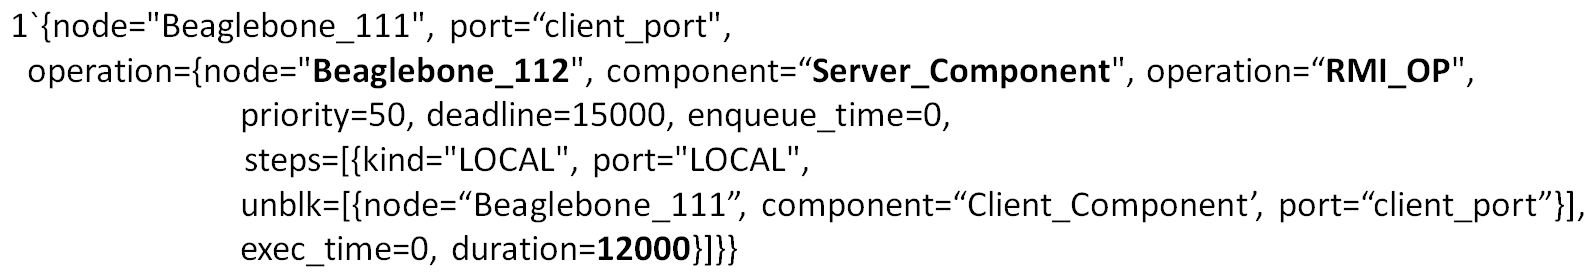
\includegraphics[width=0.5\textwidth]{cpn_rmi_app_iop}
\caption{Operation Induction Token}
\label{fig:cpn_rmi_app_iop}
\vspace{-0.16in}
\end{figure}

In this token, \emph{i\_call\_id = 1} represents the RMI call on the client. When the client thread is the currently running thread, it runs for as long as required to push out the RMI query. At this point, the \emph{Induce} transition becomes enabled and the RMI operation \emph{i\_op} is placed in \emph{Waiting for Enqueue}, eventually getting serviced. When initializing the model, a token is placed on \emph{Induce Operation} for every component interaction in the system, all of which are known ahead of time when the developer designs the application.
\section{State Space Analysis}
\label{sec:State_Space_Analysis}

In order to describe the utility of state space-based analysis, we consider the simplified version of a trajectory planning application requiring strict temporal behavior. The component assembly for this application is shown in Figure \ref{fig:tpa}. This application consists of two components: A \emph{Sensor} component and a \emph{Trajectory Planner} component. The Sensor component periodically publishes on a trigger topic, notifying the Trajectory Planner of the existence of new sensor data. Once the notification is received, the Trajectory Planner makes an RMI call to retrieve the data structure of sensor values. Using the updated sensor values, the Trajectory Planner calculates a new trajectory for the satellite. 

\begin{figure}[ht]
\centering
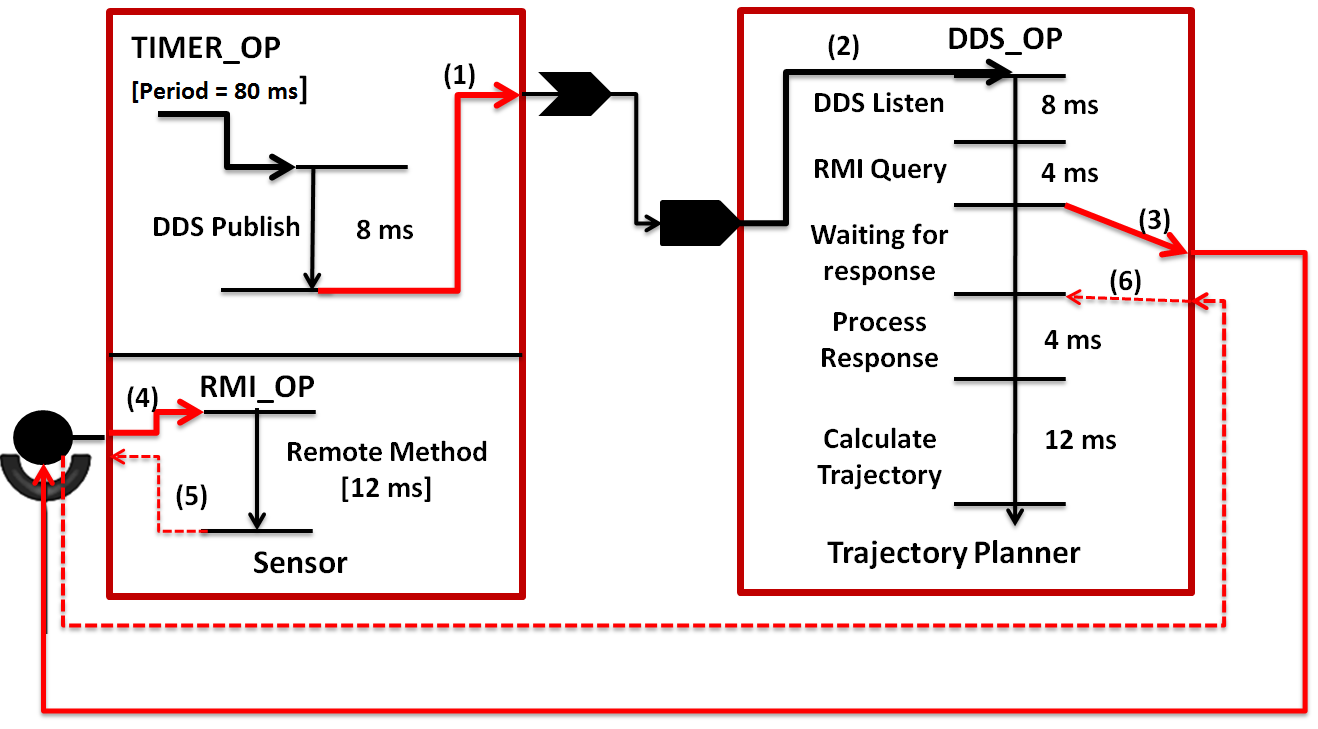
\includegraphics[width=0.5\textwidth]{tpa}
\caption{Trajectory Planning Application}
\label{fig:tpa}
\vspace{-0.2in}
\end{figure}
%\vspace{0.1in}

\begin{figure}[ht]
\centering
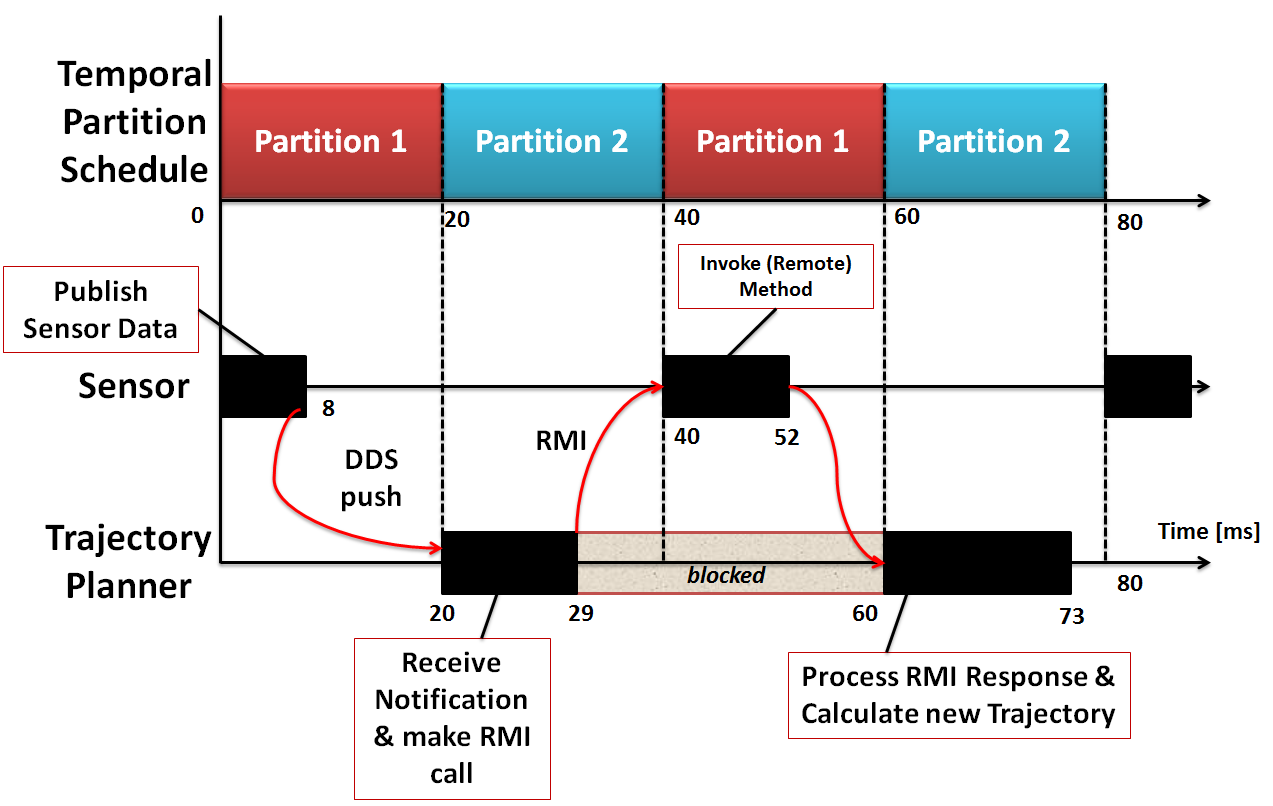
\includegraphics[width=0.5\textwidth]{tpa_td}
\caption{Timing Diagram for Trajectory Planning}
\label{fig:tpa_td}
\vspace{-0.2in}
\end{figure}
\vspace{0.1in}

Figure \ref{fig:tpa_td} shows the partition schedule and temporal behavior considered. The sensor component operates on partition 1, and the trajectory planner operates on partition 2. Both partitions have a duration of 20 ms and a period of 40 ms. The sensor component is associated with a periodic timer that fires every 80 ms. When this timer expires, the sensor component publishes on a notification topic. Accounting for network latencies, the analysis assumes that this task does not take more than 8 ms. Once the notification is sent out, the sensor component becomes passive. With DDS push semantics, this notification manifests itself as a DDS operation on the trajectory planner's message queue. When partition 2 becomes active, the trajectory planner component receives the notification is has subscribed to, after which it makes an RMI call to the sensor component to obtain the updated sensor values. After the RMI call is made, this component blocks for the remainder of the partition. When the sensor component is scheduled again, it services the RMI request and sends out the RMI response, effectively unblocking the trajectory planner. Once the new sensor data is retrieved, the trajectory planner calculates a new trajectory for the satellite node. %	For the sake of analysis, we assume the temporal behavior shown in Figure \ref{fig:tpa}.

%Using the in-built state space tool, a complete or partial state space can be generated for the modeled system. Partial state spaces are generated by specifying predicates or limiting paramters e.g. number of state space nodes. Once generated, a standard report summarizes the results. This report provides information  on: (1) Size of the state space, (2) Boundedness Properties for all the places in the model, (3) Liveness Properties for all transitions in the model, (4) Fairness Properties for transition  firings, and (5) Home Properties for home markings. It is, however, not necessary to generate this report as all of this information can be derived using the \emph{Evaluate ML} feature in CPN Tools. Here, state space queries are written as auxiliary text in the model and evaluated as standard ML code. 

%\vspace{-0.15in}
\subsection{Deadline Violation Detection}

Using the \emph{op\_st} and \emph{op\_et} fields of every component operation, the model is capable of identifying deadline violations in component operations that are either currently in progress or waiting in the component message queue. The model essentially takes a snapshot of such cases and records the time stamps. For instance: In Figure \ref{fig:tpa_td}, the \emph{DDS\_OP} on the Trajectory Planner Component starts at time = 20 and completes at time = 73, taking 53 ms accounting for temporal partitioning and the block time due to the remote call. If the deadline for this operation were to be set at 40 ms, the model would take notice of the violation at time = 61. This can also be observed by relying on the simulation tool as there is only one thread execution order for this scenario. Figures \ref{fig:cpn_tpa_dv_marking} and \ref{fig:cpn_tpa_dv_ss} show the observed deadline violation and the state space queries that reinforce the observation. The \emph{SearchNodes} function enables searching parts of the state space and identifying nodes that support a predicate function. In this case, the predicate function obtains state space nodes where a deadline violation is recorded in the \emph{Late\_Operations} place. From this subset of nodes, unique deadline violations are identified. A backtrace for the observed violation can be easily obtained by using the \emph{NodesInPath (InitialNode, DestNode)} function that presents an ordered list of state space nodes from the initial node that represents the path taken to reach the violation node.

\begin{figure}[ht]
\centering
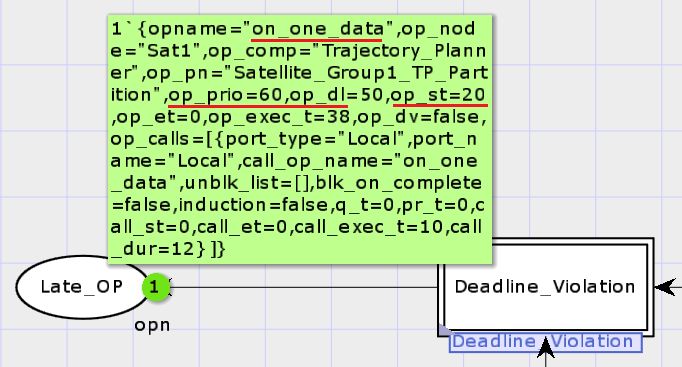
\includegraphics[width=0.29\textwidth]{cpn_tpa_dv_marking}
\caption{Observed Deadline Violation}
\label{fig:cpn_tpa_dv_marking}
\vspace{-0.2in}
\end{figure}
\vspace{0.1in}

\begin{figure}[ht]
\centering
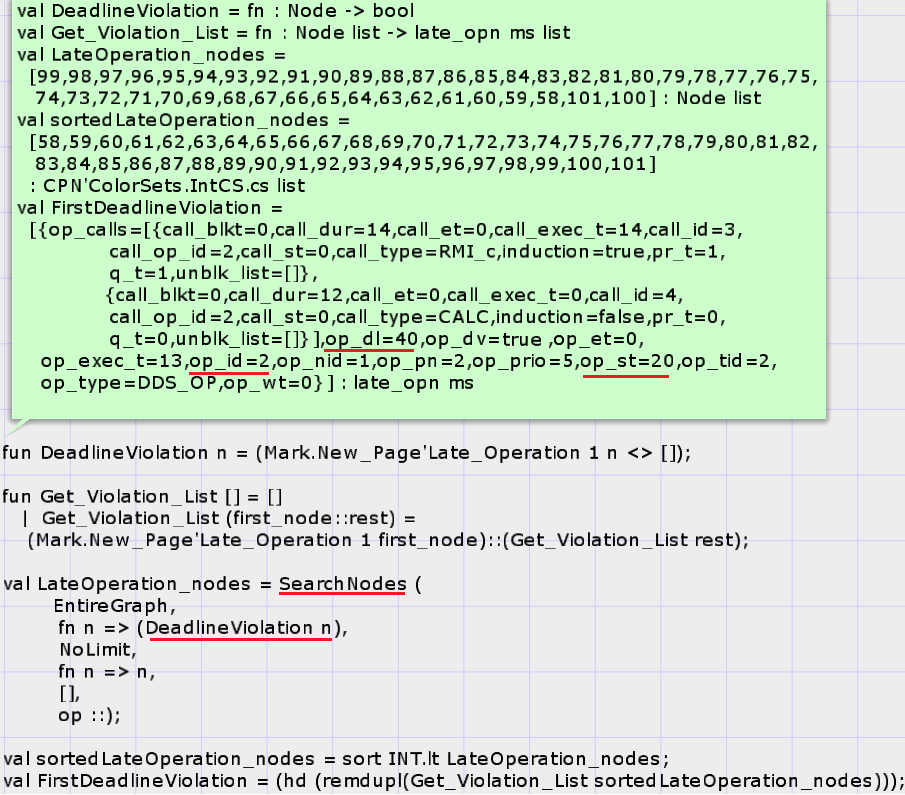
\includegraphics[width=0.5\textwidth]{cpn_tpa_dv_ss}
\caption{State Space Query for Deadline Violation Detection}
\label{fig:cpn_tpa_dv_ss}
\vspace{-0.2in}
\end{figure}
%\vspace{0.1in}

\subsection{Worst-case Trigger-to-Response Time Calculation}

As component operations run to completion, the analysis model keeps track of operation completion using a \emph{Completed\_Operations} place as shown in Figure \ref{fig:cpn_completed_operations}. 

\begin{figure}[ht]
\centering
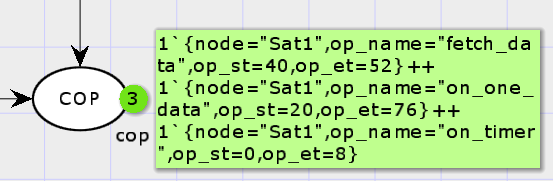
\includegraphics[width=0.35\textwidth]{cpn_completed_operations}
\caption{Completed Operations}
\label{fig:cpn_completed_operations}
\vspace{-0.2in}
\end{figure}
\vspace{0.1in}

For a known trigger operation and desired response operation, the worst-case trigger-to-response time can also be calculated from the generated state space. This is especially useful when multiple threads of same priority share a partition leading to a tree of possible thread execution orders. Once the necessary partial state space is generated, by using the operation IDs of the trigger and response, the earliest completion of the trigger operation and the latest completion of the response operation within the set period are identified. In the Trajectory Planning application, considering the \emph{TIMER\_OP} (\emph{op\_id = 1}) to be the trigger and the trajectory planning \emph{DDS\_OP} to be the response, the worst-case response time is found to be 65 ms as shown in Figure \ref{fig:cpn_tpa_trigger_response_time}. Since all of the necessary information is already packed in the state space, variants of such queries can be easily constructed without changing the model.

\begin{figure}[ht]
\centering
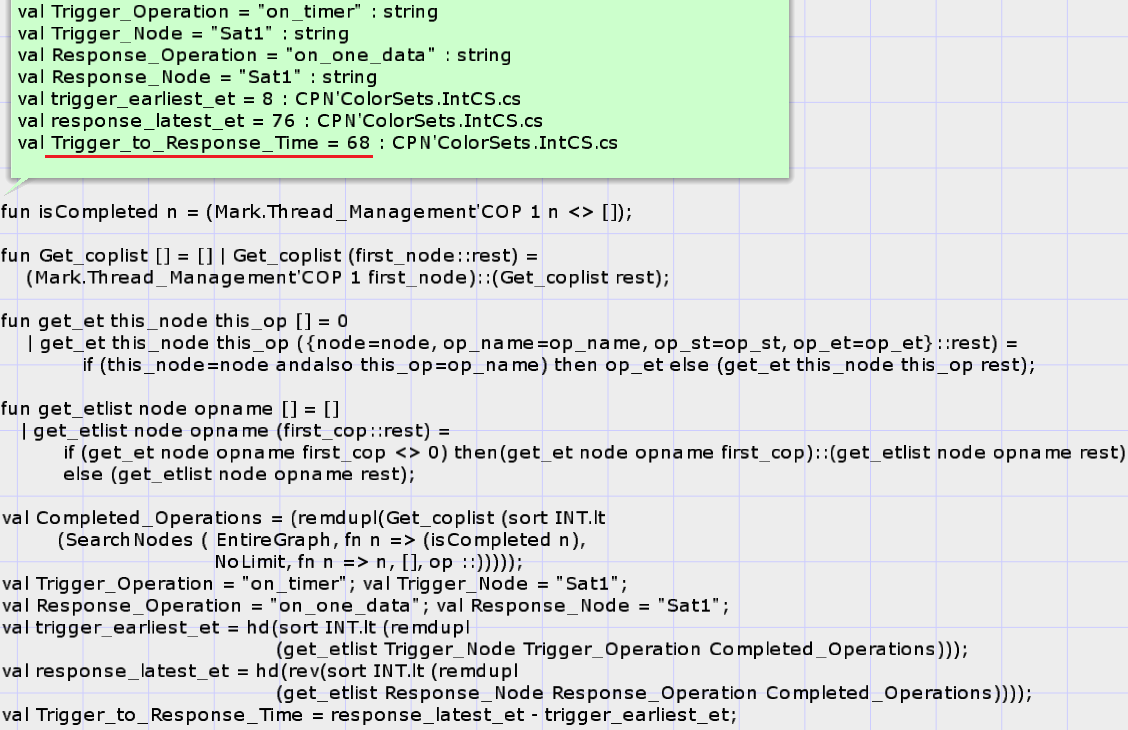
\includegraphics[width=0.5\textwidth]{cpn_tpa_trigger_response_time}
\caption{Worst-Case Trigger-to-Response Time Calculation}
\label{fig:cpn_tpa_trigger_response_time}
\vspace{-0.2in}
\end{figure}
\vspace{0.1in}

\subsection{Partial Thread Execution Order Generation}

Since the start and end time stamps of any completed operation can be obtained from the state space, this feature can be exploited to obtain a partial thread execution order and therefore thread priorities for applications in the design process. Consider the sample application shown in Figure \ref{fig:partial_order_example}.

\vspace{-0.08in}
\begin{figure}[ht]
\centering
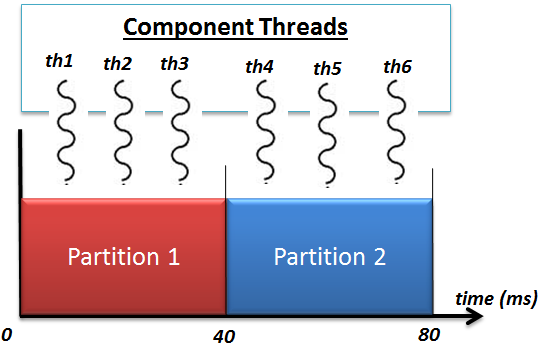
\includegraphics[width=0.25\textwidth]{partial_order_example}
\caption{Sample Application in Design Process}
\label{fig:partial_order_example}
\vspace{-0.16in}
\end{figure}

This application consists of 6 component executor threads that service component operation requests. Threads 1, 2, and 3 are assigned to Partition 1 and threads 4, 5, and 6 are assigned to Partition 2. The thread priorities and execution orders are unknown. Each component is associated with a timer that triggers an operation once every major frame, taking up to 8 ms to complete. The design requires that operation 3 (handled by thread 3) must complete before 20 ms and operation 5 (handled by thread 5) must complete before 60 ms from start of schedule. Figure \ref{fig:cpn_partial_order} shows queries that use the generated state space to obtain a thread execution order that satisfies such timing constraints. All threads are assigned the same priority and scheduling is therefore Round-Robin. The generated state space (size = 5000 nodes) records all possible thread execution orders for one hyperperiod of the schedule. From this partial state space, the state space node that first satisfies the timing requirement is identified. By generating a backtrace from the initial node and identifying the subset of nodes where the system clock ticks, the thread execution order is determined. It is clear that as the timing requirements become stricter, the number of possible thread execution orders decrease. For multiple timing requirements, if the set of thread execution orders contradict each other, the order that satisfies the higher priority timing requirement is chosen.

\vspace{-0.08in}
\begin{figure}[ht] 
\centering
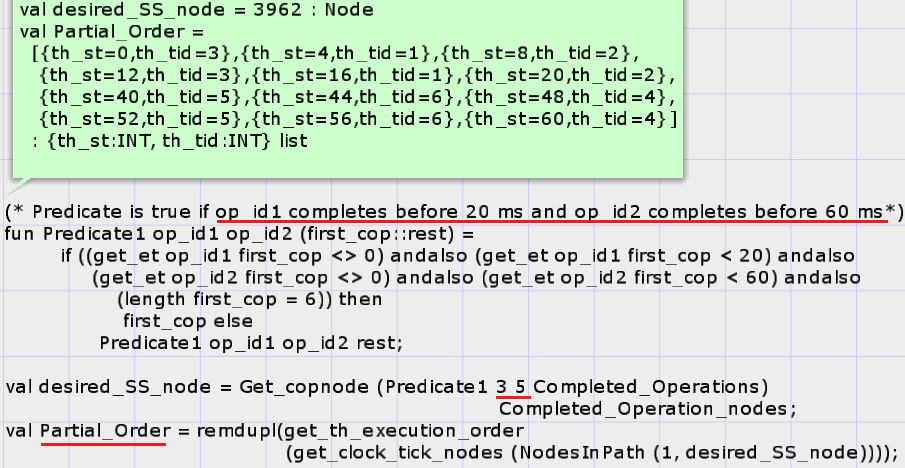
\includegraphics[width=0.5\textwidth]{cpn_partial_order}
\caption{Partial Order for Thread Execution}
\label{fig:cpn_partial_order}
\vspace{-0.18in}
\end{figure}

\subsection{Scalability Testing}
\label{subsec:Scalability_Testing}

The size of the generated state space is dependent on the amount of concurrency in the behavior. If all the executing threads had unique priorities, the thread execution order is a constant as the scheduling is priority-based. However, for larger systems with multiple applications and with threads of same priority sharing processor time in the same partition, several thread execution orders are possible depending on the arrival rates of operation requests and state of executing threads.  

Consider a set of mixed-criticality applications deployed on a 3-node satellite cluster. Each node has a unique temporal partition schedule with the longest schedule having a hyperperiod of 1 second, spanning 5 partitions. Hundred threads within the priority range [30-90] are distributed across the nodes. Most of the application component threads are triggered by timers of varying periodicity. In order to maximize the concurrency and possibilities of thread execution orders, most of the application threads are assigned the same priority and are also completely independent of each other. Dependence between components forces certain thread execution behaviors and so this is avoided. The Analysis model has 14 transitions and 11 places of which 3 places are observer places. Structural reductions to the model further reduce the state space size. Table \ref{tbl:scalability} summarizes the results of this effort. One of the observed consequences for such large systems is that the CPN Tools user interface suffers a rendering lag when it has to keep track of and display large token sets. This can be avoided by hiding as much detail as possible using hierarchy. 

\begin{table}[htbp]
\centering
\caption{Scalability Testing}
\begin{tabular}{| c | c | c | c | p{1.3cm} |}
\hline
 Satellites & Threads & Hyperperiods & State Space Nodes \\\hline
%TPA & 1 & 2 & 10 & 1500 \\\hline
%TPA & 2 & 2 & 10 & 3500 \\\hline
%TPA & 3 & 2 & 10 & 15000 \\\hline
%TPA & 4 & 2 & 10 & 30000 \\\hline
%TPA & 5 & 2 & 10 & 90000 \\\hline
1 & 50 & 10 & 125,000 \\\hline
3 & 100 & 10 & 480,000 \\\hline
\end{tabular}
\label{tbl:scalability}
\end{table}
\vspace{-0.1in}

\section{Analysis Model Generation}
\label{sec:Model_Generation}

For large applications, with several timers and component interaction patterns, hand-writing the CPN token specification will prove to be cumbersome and error prone. This can be avoided by integrating the temporal behavior specification for component-based applications onto the modeling framework used to generate the deployment plans and infrastructure glue code, effectively closing the loop shown in Figure \ref{fig:big_picture}. Since the structure of the places, transitions, color-sets, variables and function declarations do not change, only the application-specific token structure needs to be derived from the design model of the application. Figure \ref{fig:model_generation} shows a part of the ANTLR-based \cite{ANTLR_BOOK} specification grammar, a part of the input text file and the generated CPN tokens. 

\begin{figure}[ht] 
\centering
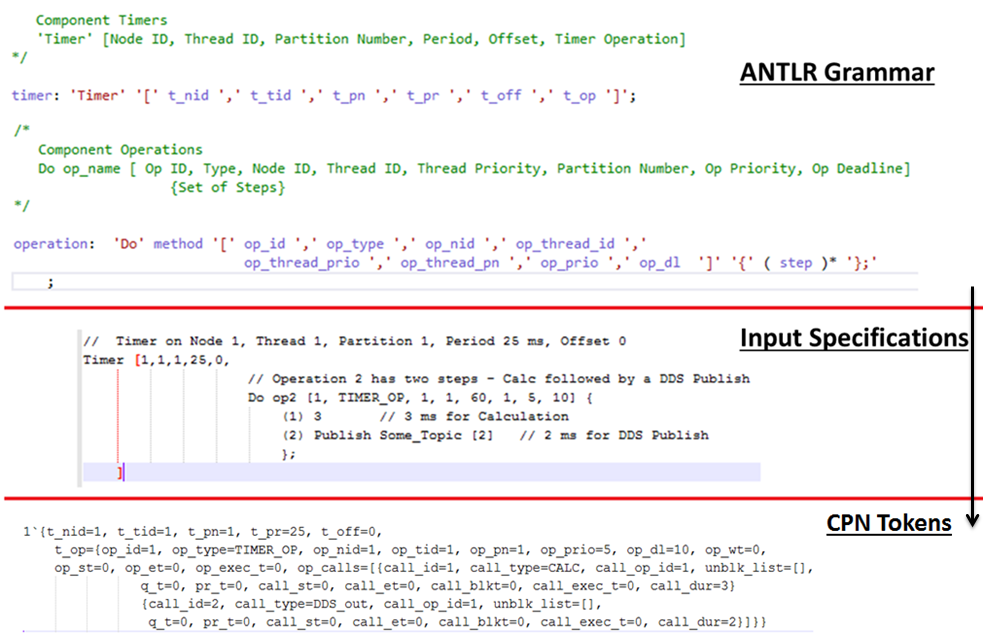
\includegraphics[width=0.5\textwidth]{model_generation}
\caption{Analysis Model Generation}
\label{fig:model_generation}
\vspace{-0.2in}
\end{figure}

\section{Discussion}
\label{sec:Discussion}

One of the main concerns in comprehensive design-time analysis of this kind is scalability. As the determinism in the initial design increases, the number of possible behaviors and therefore the size of the state space decreases. In essence, the effort required for the analysis to be useful for a designer is dependent heavily on the initial design itself. With increasing number of timer operations and equal priority threads sharing a CPU, the number of possible thread execution orders and behavioral scenarios will exponentially grow, leading to unmanageable state space sizes. The results shown in Table \ref{tbl:scalability} do not represent an upper bound on the state space size but one corresponding to an average-case scenario. For safety-critical systems, deterministic system behavior requires deterministic system designs. Since worst-case estimates are considered, it is unlikely that the actual system behavior would even reach certain behavioral regions. Therefore, the analysis results obtained from this approach effectively behave as guidelines for a more refined, and predictable application design as opposed to hard constraints on possible design.  

\section{Future Work}
\label{sec:Future_Work}

In order to generalize this analysis model and provide flexibility, one possible extension to this approach is to cater to other commonly used scheduling schemes such as EDF, RMS etc. for component operation scheduling; and novel interaction patterns (e.g. reliable broadcast). Since the analysis model is a composition of sub-nets that are not tightly coupled, this extension would provide reusable, self-contained functional modules. 

The current analysis approach inherits the benefits and the drawbacks of using pessimistic estimates for execution times. Another possible extension to this approach would be to provide a stochastic schedulability analysis allowing for a trade-off between reliability and cost of resources required by the system. However, describing execution times for software using probability distribution functions is not trivial and would require significant effort.

\section{Conclusions}
\label{sec:Conclusions}

Mobile, distributed real-time systems operating in dynamic environments, and running mission-critical applications face strict timing requirements to operate safely. To reduce the development and integration complexity for such systems, component-based design models are being increasingly used. Appropriate analysis models are required to study the structural and behavioral complexity in such designs. 

This paper presents a Colored Petri net-based approach to capture the architecture and temporal behavior of such component-based applications for both qualitative and quantitative schedulability analysis. This analysis model includes a compact, scalable representation of high-level design, accounting for the dynamics of real-time thread execution while exploiting knowledge of component execution code. Exhaustive state space search enables verification and validation of useful and necessary system properties, reducing development costs and increasing reliability for such time-critical systems. The utility of this tool has been illustrated with several examples. 

\textbf{Acknowledgments:} The DARPA System F6 Program and the National
Science Foundation (CNS-1035655) supported
this work. Any opinions, findings, and conclusions or recommendations expressed
in this material are those of the authors and do not reflect the views of
DARPA or NSF. 

%This work was supported by the DARPA System F6 Program
%under contract NNA11AC08C and the National Science Foundation (CNS-1035655). Any opinions, findings, and
%conclusions or recommendations expressed in this material
%are those of the author(s) and do not  reflect
%the views of DARPA or NSF. The authors thank Olin Sibert of Oxford
%Systems and all the team members of our project for their
%invaluable input and contributions to this effort.

%The DARPA System F6 Program and the National Science Foundation (CNS-1035655) supported this work. Any opinions, findings, and conclusions or recommendations expressed in this material are those of the authors and do not reflect the views of DARPA or NSF. 
%\vspace{-0.1in}
\balance
\begin{spacing}{0.88}
\bibliographystyle{IEEEtran}
\bibliography{../bibliography/f6}
\end{spacing}

\end{document}
